% =====================================================================
%  Chapitre 3 -- Architecture d'un reseau convolutif
%  Partie c : LeNet, architectures historiques, blocs residuels, quiz
% =====================================================================

\begin{frame}{LeNet-5 (LeCun, 1998) : le premier CNN opérationnel}
\begin{columns}[t]
\begin{column}{0.48\textwidth}
\centering
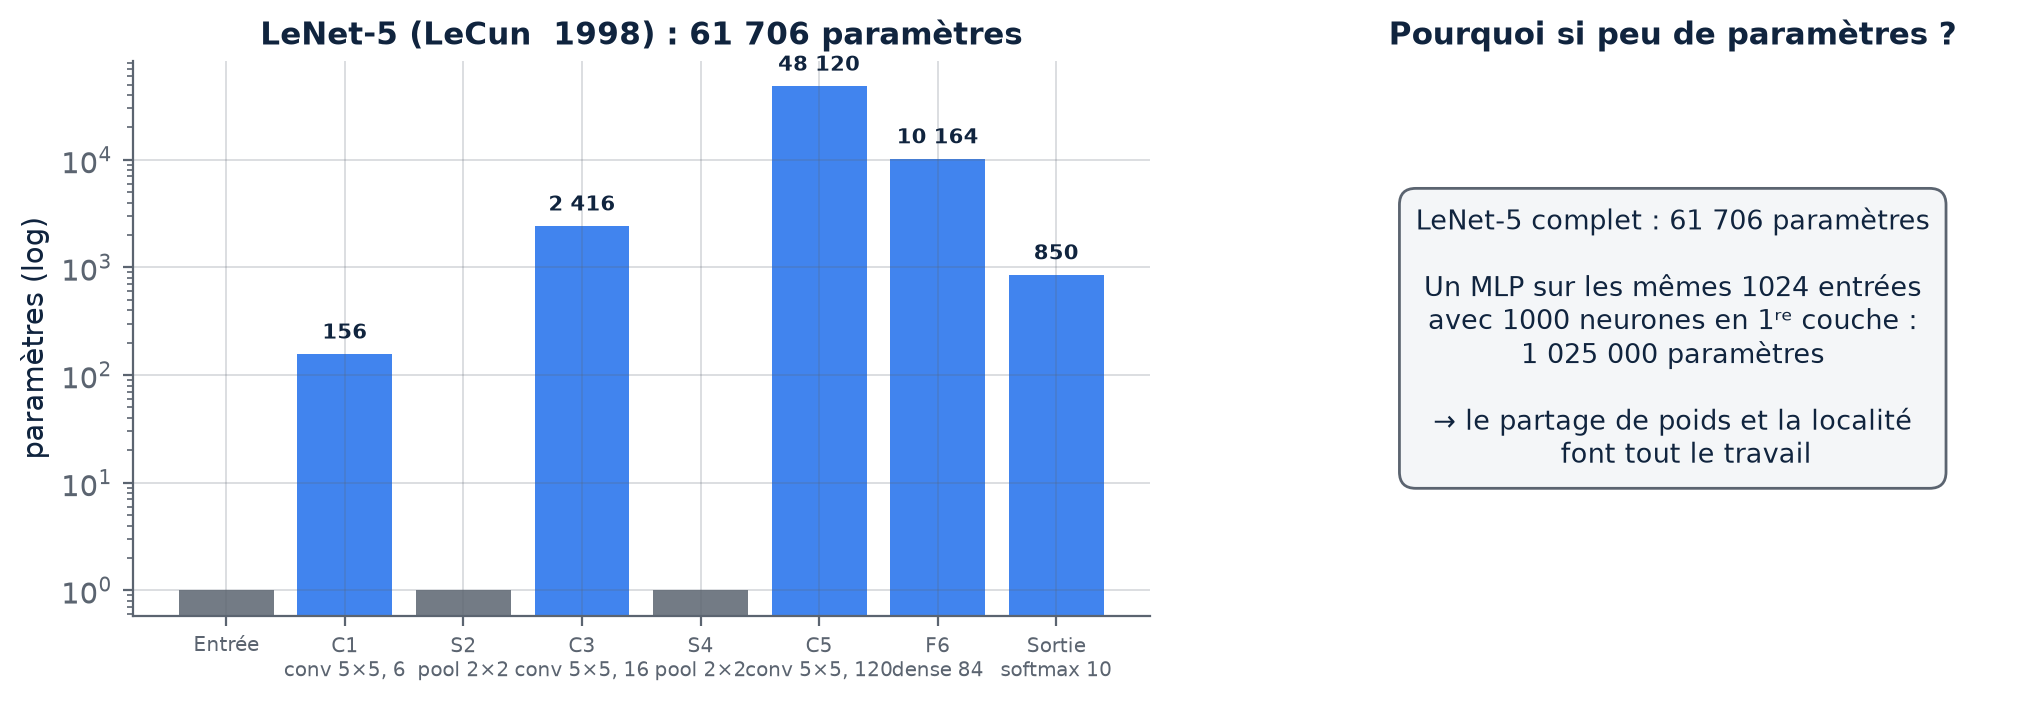
\includegraphics[width=0.46\textwidth]{h05_lenet.png}
\end{column}
\begin{column}{0.48\textwidth}
\begin{itemize}
  \item LeNet-5 est conçu pour lire les \textbf{chiffres manuscrits}
  (chèques bancaires, code postal).
  \item Entrée : une petite image en niveaux de gris de $32 \times 32$.
  \item Sortie : \textbf{10 classes} (les chiffres de 0 à 9).
  \item Toute l'architecture tient en \textbf{7 couches} : conv, pool,
  conv, pool, conv, dense, sortie.
\end{itemize}
\begin{kbox}[Ce qui fait sa force]
Trois idées seulement : \textbf{localité} (petits noyaux $5\times5$),
\textbf{partage de poids} (le même filtre sur toute l'image) et
\textbf{sous-échantillonnage} (pooling).
\end{kbox}
\end{column}
\end{columns}
\end{frame}

\begin{frame}{LeNet-5 : couche par couche (entrée $\rightarrow$ S4)}
\begin{columns}[t]
\begin{column}{0.48\textwidth}
\begin{itemize}
  \item \textbf{Entrée} : $32 \times 32 \times 1$.
  \item \textbf{C1} --- convolution $5\times5$, \textbf{6 filtres} :
  la carte rétrécit de $2$ de chaque côté.
  \begin{itemize}
    \item Sortie : $28 \times 28 \times 6$.
    \item Paramètres : $(5\cdot 5\cdot 1 + 1)\times 6 = \mathbf{156}$.
  \end{itemize}
  \item \textbf{S2} --- pooling max $2\times2$, pas de $2$ :
  \begin{itemize}
    \item Sortie : $14 \times 14 \times 6$.
    \item \textbf{0 paramètre} : le pooling n'apprend rien.
  \end{itemize}
\end{itemize}
\end{column}
\begin{column}{0.48\textwidth}
\begin{itemize}
  \item \textbf{C3} --- convolution $5\times5$, \textbf{16 filtres} sur
  les 6 canaux précédents.
  \begin{itemize}
    \item Sortie : $10 \times 10 \times 16$.
    \item Paramètres : $(5\cdot 5\cdot 6 + 1)\times 16 = \mathbf{2\,416}$.
  \end{itemize}
  \item \textbf{S4} --- pooling max $2\times2$ :
  \begin{itemize}
    \item Sortie : $5 \times 5 \times 16$.
    \item \textbf{0 paramètre}.
  \end{itemize}
\end{itemize}
\begin{kbox}[Deux étages, deux rôles]
La convolution \textbf{extrait} des motifs ; le pooling \textbf{résume}
et réduit la taille. Ce duo se répète tout au long du réseau.
\end{kbox}
\end{column}
\end{columns}
\end{frame}

\begin{frame}{LeNet-5 : couche par couche (C5 $\rightarrow$ sortie)}
\begin{columns}[t]
\begin{column}{0.52\textwidth}
\begin{itemize}
  \item \textbf{C5} --- convolution $5\times5$, \textbf{120 filtres} :
  l'entrée ne fait que $5\times5$, la carte devient $1\times1$.
  \begin{itemize}
    \item Sortie : $1 \times 1 \times 120$.
    \item Paramètres : $(5\cdot 5\cdot 16 + 1)\times 120 = \mathbf{48\,120}$.
  \end{itemize}
  \item \textbf{F6} --- couche dense de \textbf{84} neurones
  (\emph{aplatissement} des 120 valeurs au préalable) :
  \begin{itemize}
    \item Paramètres : $120 \times 84 + 84 = \mathbf{10\,164}$.
  \end{itemize}
  \item \textbf{Sortie} --- dense de \textbf{10} neurones avec \emph{softmax} :
  \begin{itemize}
    \item Paramètres : $84 \times 10 + 10 = \mathbf{850}$.
  \end{itemize}
\end{itemize}
\end{column}
\begin{column}{0.44\textwidth}
\begin{ebox}[Observation importante]
La convolution $5\times5$ appliquée à une carte $5\times5$ produit
\emph{un seul} nombre par filtre : c'est une manière élégante de passer
d'un \textbf{tenseur} à un \textbf{vecteur} sans jeter la structure.
\end{ebox}
\begin{wbox}[Le piège de la dernière couche]
C'est ici que se concentrent les paramètres denses : F6 et la sortie
pèsent à eux deux $10\,164 + 850 = \mathbf{11\,014}$ paramètres,
soit près d'un cinquième du total.
\end{wbox}
\end{column}
\end{columns}
\end{frame}

\begin{frame}{LeNet-5 : tableau récapitulatif}
\begin{center}
\small
\begin{tabular}{@{}llrr@{}}
\toprule
\textbf{Couche} & \textbf{Opération} & \textbf{Sortie (h$\times$w$\times$c)}
 & \textbf{Paramètres} \\
\midrule
Entrée   & image               & $32 \times 32 \times 1$  & 0 \\
C1       & conv $5\times5$, 6  & $28 \times 28 \times 6$  & 156 \\
S2       & pool max $2\times2$ & $14 \times 14 \times 6$  & 0 \\
C3       & conv $5\times5$, 16 & $10 \times 10 \times 16$ & 2\,416 \\
S4       & pool max $2\times2$ & $5 \times 5 \times 16$   & 0 \\
C5       & conv $5\times5$, 120& $1 \times 1 \times 120$  & 48\,120 \\
F6       & dense 84            & $1 \times 1 \times 84$   & 10\,164 \\
Sortie   & dense 10 + softmax  & $1 \times 1 \times 10$   & 850 \\
\midrule
\multicolumn{3}{r}{\textbf{Total}} & \textbf{61\,706} \\
\bottomrule
\end{tabular}
\end{center}
\vspace{1mm}
\begin{kbox}[À retenir]
Un CNN de $62\,000$ paramètres à peine reconnaît les chiffres manuscrits :
par comparaison, un MLP direct sur $32\times32$ en exigerait plusieurs
centaines de milliers, sans aucune garantie d'invariance par translation.
\end{kbox}
\end{frame}

\begin{frame}[fragile]{D'où viennent ces nombres ? La formule des paramètres}
\begin{columns}[t]
\begin{column}{0.50\textwidth}
\begin{itemize}
  \item Une couche convolutive n'apprend que le \textbf{noyau} et le
  \textbf{biais} : elle les \emph{réutilise} sur toute l'image.
  \item Nombre de paramètres d'une convolution :
  \[
    \underbrace{(k_h \cdot k_w \cdot c_{in})}_{\text{poids}} + 1
    \quad\text{par filtre,}
  \]
  multiplié par le nombre de filtres $c_{out}$.
  \item Une couche dense, elle, dépend de la \emph{taille} de l'entrée :
  \[
    n_{in} \cdot n_{out} + n_{out}.
  \]
\end{itemize}
\end{column}
\begin{column}{0.46\textwidth}
\begin{codebox}[Compter les paramètres en Python]
\begin{lstlisting}
def params_conv(k, c_in, c_out):
    poids = k * k * c_in
    return (poids + 1) * c_out

def params_dense(n_in, n_out):
    return n_in * n_out + n_out

# C1, C3, C5 de LeNet-5
print(params_conv(5, 1, 6))    # 156
print(params_conv(5, 6, 16))   # 2416
print(params_conv(5, 16, 120)) # 48120

# F6 et la sortie
print(params_dense(120, 84))   # 10164
print(params_dense(84, 10))    # 850
\end{lstlisting}
\end{codebox}
\end{column}
\end{columns}
\end{frame}

\begin{frame}{LeNet-5 : un coût minuscule comparé au dense}
\begin{columns}[t]
\begin{column}{0.48\textwidth}
\begin{itemize}
  \item Un MLP qui prendrait directement les $32\times32 = 1\,024$ pixels
  en entrée et les connecterait à 84 neurones :
  \[
    1\,024 \times 84 + 84 = \mathbf{86\,100}
  \]
  paramètres rien que pour \emph{une} couche.
  \item LeNet-5 fait tout le travail d'extraction avec environ
  \textbf{62\,000} paramètres.
\end{itemize}
\begin{kbox}[Deux régimes de coût]
Le convolutif coûte $k^2 \cdot c_{in}$ \textbf{par filtre}, indépendamment
de la taille de l'image. Le dense coûte $n_{in} \cdot n_{out}$, proportionnel
à la surface de l'entrée.
\end{kbox}
\end{column}
\begin{column}{0.48\textwidth}
\begin{ebox}[Et sur une grande image ?]
Une photo $1\,000 \times 1\,000$ en couleur ($3$ canaux) connectée à
84 neurones denses exigerait
$3\,000\,000 \times 84 + 84 = \mathbf{252\,000\,084}$ paramètres
pour \emph{une seule} couche.

\medskip
La même couche, en convolution $5\times5$ avec $16$ filtres, n'en
demande que $(5\cdot 5\cdot 3 + 1)\times 16 = \mathbf{1\,216}$ :
le sujet du chapitre 1, chiffré.
\end{ebox}
\end{column}
\end{columns}
\end{frame}

\begin{frame}{Les grandes architectures historiques}
\begin{columns}[t]
\begin{column}{0.56\textwidth}
\centering
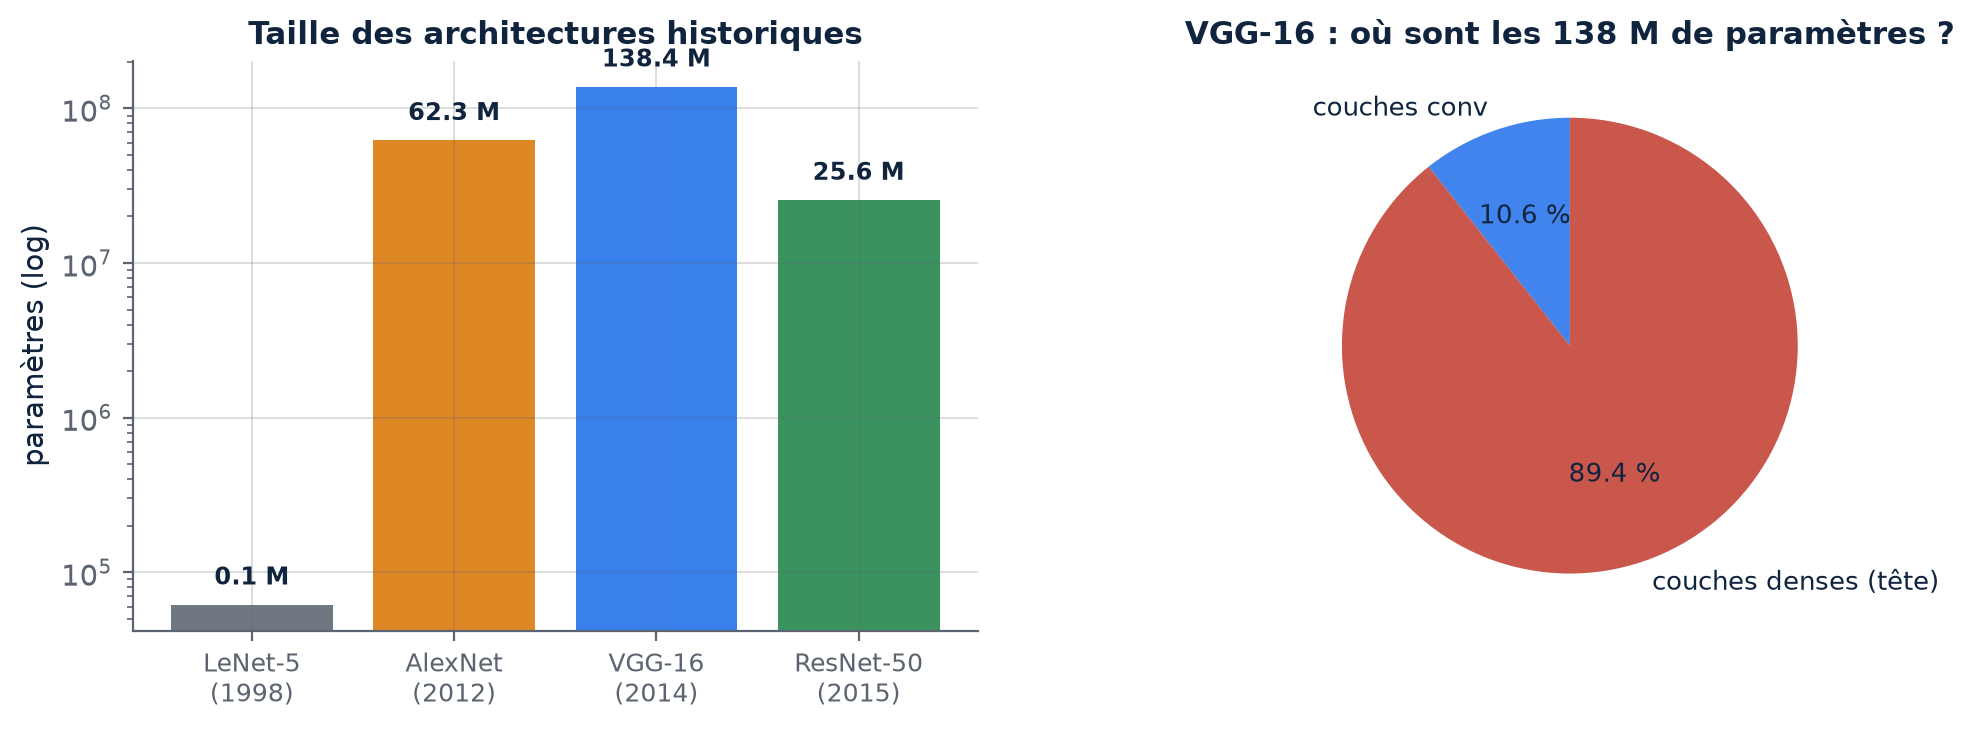
\includegraphics[width=0.54\textwidth]{h06_architectures.png}
\end{column}
\begin{column}{0.40\textwidth}
\begin{itemize}
  \item \textbf{LeNet-5} (1998) : $7$ couches, conv $5\times5$, déjà
  toutes les briques des CNN modernes.
  \item \textbf{AlexNet} (2012) : la profondeur explose, entraînée sur GPU.
  \item \textbf{VGG} (2014) : noyaux $3\times3$ empilés jusqu'à 19 couches.
  \item \textbf{ResNet} (2015) : les connexions sautées font tomber la
  barrière de la profondeur (plus de 100 couches).
\end{itemize}
\end{column}
\end{columns}
\end{frame}

\begin{frame}{AlexNet (2012) : le basculement}
\begin{columns}[t]
\begin{column}{0.50\textwidth}
\begin{itemize}
  \item Vainqueur d'ImageNet 2012 avec une marge sans précédent
  (erreur divisée par près de deux face au second).
  \item Environ \textbf{62 millions} de paramètres, bien loin des
  $62$ milliers de LeNet.
  \item Entrée bien plus grande que LeNet : images couleur $227\times227$.
  \item En 2012, c'est le \textbf{GPU} qui rend l'entraînement possible.
\end{itemize}
\end{column}
\begin{column}{0.46\textwidth}
\begin{kbox}[Les trois nouveautés d'AlexNet]
\begin{itemize}
  \item \textbf{ReLU} : activation non saturante, qui accélère
  fortement la convergence face à la sigmoïde.
  \item \textbf{Dropout} : des neurones tirés au sort à chaque passe,
  pour lutter contre le surapprentissage.
  \item \textbf{GPU} : entraîner deux réseaux parallèles sur cartes graphiques.
\end{itemize}
\end{kbox}
\begin{ebox}[La leçon]
AlexNet n'invente presque rien : il \emph{assemble}.
Conv + ReLU + pool + dropout + beaucoup de données + GPU $=$ la
révolution de l'apprentissage profond.
\end{ebox}
\end{column}
\end{columns}
\end{frame}

\begin{frame}{VGG-16 (2014) : la profondeur comme principe}
\begin{columns}[t]
\begin{column}{0.48\textwidth}
\begin{itemize}
  \item Un principe unique : \textbf{n'utiliser que des noyaux $3\times3$},
  empilés, avec un pooling $2\times2$ tous les deux ou trois blocs.
  \item $16$ couches avec poids : beaucoup plus profond qu'AlexNet,
  mais plus simple à décrire.
  \item Idée clé : deux convolutions $3\times3$ empilent un champ
  récepteur de $5\times5$, avec \textbf{moins} de poids et une activation
  de plus.
  \item L'architecture de référence pour le \emph{transfert learning}
  (chapitre 4).
\end{itemize}
\end{column}
\begin{column}{0.48\textwidth}
\begin{wbox}[Le coût caché de VGG-16]
\textbf{138\,357\,544} paramètres au total, dont :
\begin{itemize}
  \item \textbf{14\,714\,688} dans les couches convolutives ;
  \item \textbf{123\,642\,856} dans les couches denses.
\end{itemize}
Autrement dit, \textbf{89{,}4 \%} des paramètres sont \emph{denses} :
l'essentiel du coût n'est pas dans la convolution.
\end{wbox}
\begin{kbox}[Le constat qui a changé les architectures]
VGG a poussé la profondeur conv, mais ce sont les dernières couches denses
qui pèsent le plus lourd. La suite -- ResNet, puis les architectures sans
couche dense -- corrige ce déséquilibre.
\end{kbox}
\end{column}
\end{columns}
\end{frame}

\begin{frame}{ResNet (2015) : entraîner des réseaux très profonds}
\begin{columns}[t]
\begin{column}{0.48\textwidth}
\begin{itemize}
  \item Observation contre-intuitive : ajouter des couches à un réseau
  « assez profond » \textbf{dégrade} la précision sur l'entraînement
  lui-même. Ce n'est pas du surapprentissage, c'est une difficulté
  d'optimisation.
  \item ResNet emprunte à VGG ses noyaux $3\times3$, mais ajoute une seule
  chose : la \textbf{connexion sautée}.
  \item Résultat : des réseaux à \textbf{plus de 100 couches} non seulement
  entraînables, mais plus précis.
\end{itemize}
\end{column}
\begin{column}{0.48\textwidth}
\begin{kbox}[Connexion sautée (\emph{skip connection})]
On ne remplace pas la sortie du bloc : on \textbf{lui ajoute l'entrée}.
\[
  y = F(x) + x
\]
Si la couche apprise $F$ est inutile, le réseau apprend simplement
$F(x)\approx 0$ et recopie $x$ : ajouter un bloc ne peut pas nuire.
\end{kbox}
\begin{ebox}[Identity mapping]
La partie $+x$ s'appelle le \emph{réseau identité} : elle laisse passer
le signal tel quel, sans le transformer.
\end{ebox}
\end{column}
\end{columns}
\end{frame}

\begin{frame}{Pourquoi $y = F(x) + x$ débloque la profondeur}
\begin{columns}[t]
\begin{column}{0.52\textwidth}
\begin{itemize}
  \item Pendant la rétropropagation, le gradient qui remonte une connexion
  sautée traverse l'identité : $\dfrac{\partial}{\partial x}(F(x)+x)
  = F'(x) + 1$.
  \item Le terme $+1$ garantit un \textbf{chemin direct} pour le gradient,
  même si $F'(x)$ devient minuscule.
  \item Sans cette porte de sortie, le gradient s'évanouit sur des dizaines
  de couches et les premières n'apprennent plus rien (\emph{vanishing
  gradient}).
  \item C'est la raison profonde pour laquelle ResNet franchit la barrière
  des $100$ couches.
\end{itemize}
\end{column}
\begin{column}{0.44\textwidth}
\begin{kbox}[Un résumé d'une ligne]
La connexion sautée transforme un empilement de couches en une
\textbf{accumulation de corrections} : chaque bloc n'a qu'à apprendre
ce qu'il \emph{manque} à la sortie précédente.
\end{kbox}
\begin{wbox}[Attention au vocabulaire]
Ne pas confondre :
\begin{itemize}
  \item \emph{skip connection} (ResNet, U-Net) : on ajoute l'entrée
  à la sortie ;
  \item \emph{pooling} : on résume une carte par un seul nombre.
\end{itemize}
Ce sont deux mécanismes entièrement différents.
\end{wbox}
\end{column}
\end{columns}
\end{frame}

\begin{frame}{La convolution $1\times1$ : réduire les canaux}
\begin{columns}[t]
\begin{column}{0.52\textwidth}
\begin{itemize}
  \item Un noyau $1\times1$ ne regarde qu'\textbf{un pixel}, mais tous ses
  \textbf{canaux} à la fois.
  \item Il ne mélange pas les pixels voisins : il mélange les canaux.
  \[
    y_c(i,j) = \sum_{c'} w_{c,c'}\,x_{c'}(i,j) + b_c
  \]
  \item C'est donc une \textbf{combinaison linéaire de canaux}, appliquée
  identiquement en chaque position.
  \item Paramètres : $c_{in} \cdot c_{out} + c_{out}$.
\end{itemize}
\end{column}
\begin{column}{0.44\textwidth}
\begin{ebox}[À quoi cela sert-il ?]
\begin{itemize}
  \item \textbf{Réduire} le nombre de canaux avant une convolution coûteuse
  ($256 \to 64$ canaux : le coût de la conv suivante chute d'autant).
  \item \textbf{Augmenter} les canaux pour créer de nouvelles combinaisons.
  \item Ajuster la profondeur d'un tenseur \textbf{sans toucher} à sa
  résolution.
\end{itemize}
\end{ebox}
\begin{kbox}[Le rôle de liaison]
Une convolution $1\times1$ est un « goulot d'étranglement » : elle compresse
l'information avant de la traiter, à moindre frais.
\end{kbox}
\end{column}
\end{columns}
\end{frame}

\begin{frame}{Les cartes d'activation : la hiérarchie des motifs}
\begin{columns}[t]
\begin{column}{0.58\textwidth}
\centering
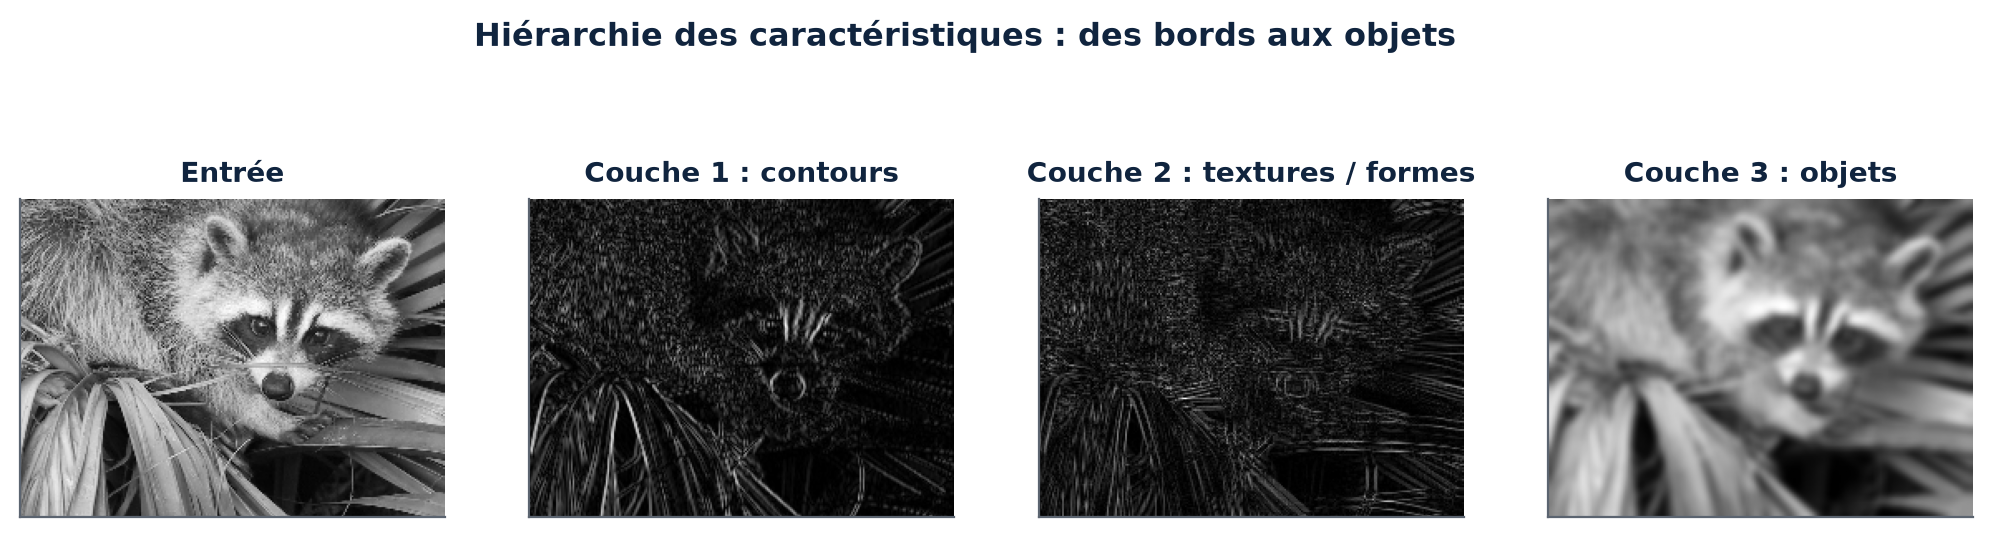
\includegraphics[width=0.56\textwidth]{h07_hierarchie_features.png}
\end{column}
\begin{column}{0.38\textwidth}
\begin{itemize}
  \item Chaque filtre produit une \textbf{carte d'activation}
  (\emph{feature map}) : la réponse du filtre en chaque position.
  \item Couches du début : \textbf{bords} et \textbf{contrastes} locaux.
  \item Couches du milieu : \textbf{textures} et \textbf{parties} de motifs.
  \item Couches profondes : \textbf{objets} entiers, puis concepts de
  haut niveau.
\end{itemize}
\end{column}
\end{columns}
\end{frame}

\begin{frame}{Lire une carte d'activation}
\begin{columns}[t]
\begin{column}{0.50\textwidth}
\begin{itemize}
  \item Une carte d'activation est une \textbf{image} : là où le motif
  cherché par le filtre est présent, les valeurs sont fortes.
  \item En superposant plusieurs cartes, on voit le réseau « regarder »
  des régions différentes.
  \item \textbf{Compter les cartes} d'une couche de convolution :
  autant que de filtres ($6$, $16$, $120$, \dots dans LeNet-5).
  \item Le \textbf{nombre de canaux} est donc une mesure directe de la
  \emph{richesse} d'une couche.
\end{itemize}
\end{column}
\begin{column}{0.46\textwidth}
\begin{kbox}[La hiérarchie bordes $\rightarrow$ objets]
\begin{center}
bords $\;\rightarrow\;$ textures $\;\rightarrow\;$ parties
$\;\rightarrow\;$ objets
\end{center}
Chaque étage \textbf{compose} ce que l'étage précédent a trouvé : c'est
exactement l'idée du Neocognitron de Fukushima (1980), rendue apprenable
par la rétropropagation.
\end{kbox}
\end{column}
\end{columns}
\end{frame}

\begin{frame}{Quiz de fin de chapitre --- questions 1 et 2}
\begin{qbox}[Question 1]
Une couche convolutive à $3$ canaux d'entrée, produisant $64$ filtres
de taille $3\times3$, avec un biais par filtre : combien de paramètres ?
\begin{itemize}
  \item[(a)] $576$ \quad (b) $1\,792$ \quad (c) $1\,856$
\end{itemize}
\end{qbox}
\begin{qbox}[Question 2]
LeNet-5 compte environ $62\,000$ paramètres. Un MLP qui prendrait les
$32\times32$ pixels en entrée et les connecterait à $84$ neurones
en utiliserait $86\,100$ \emph{pour une seule couche}. Quelle est la
conséquence ?
\begin{itemize}
  \item[(a)] Le MLP serait meilleur car plus de paramètres \\
  (b) La convolution \emph{partage} ses poids, donc coûte indépendamment
  de la taille de l'image \\
  (c) Les deux architectures coûtent le même nombre d'opérations
\end{itemize}
\end{qbox}
\end{frame}

\begin{frame}{Quiz de fin de chapitre --- questions 3, 4 et 5}
\begin{qbox}[Question 3]
À quoi sert le \emph{pooling} dans un réseau convolutif ?
\end{qbox}
\begin{qbox}[Question 4]
Qu'apporte une connexion sautée dans un réseau très profond ?
\end{qbox}
\begin{qbox}[Question 5]
Que fait exactement une convolution $1\times1$ avec $256$ canaux en entrée
et $64$ en sortie ?
\end{qbox}
\end{frame}

\begin{frame}{Réponses du quiz}
\begin{solbox}[Solutions --- à ne lire qu'après avoir répondu]
\textbf{1.} (b) : $(3\cdot 3\cdot 3 + 1)\times 64 = 28 \times 64 = 1\,792$
paramètres. \\[1mm]
\textbf{2.} (b) : un filtre convolutif n'apprend que son noyau, réutilisé
en tout point ; son coût ne dépend pas de la taille de l'image, contrairement
à la couche dense. \\[1mm]
\textbf{3.} Le pooling \textbf{ réduit la résolution} spatiale (division par
la taille de la fenêtre) et \textbf{introduit une petite invariance} aux
micro-déplacements ; il n'apprend \textbf{aucun} paramètre. \\[1mm]
\textbf{4.} La connexion sautée ajoute l'entrée à la sortie ($y = F(x)+x$).
Elle crée un \textbf{chemin direct} pour le gradient ($+1$ dans la dérivée),
ce qui évite l'évanouissement du gradient et permet d'entraîner plus de
$100$ couches. \\[1mm]
\textbf{5.} Elle combine linéairement les $256$ canaux en chaque position
pour en produire $64$ : c'est une \textbf{réduction de canaux} (goulot
d'étranglement), pour $256 \times 64 + 64 = 16\,448$ paramètres.
\end{solbox}
\end{frame}

\begin{frame}{À retenir --- chapitre 3}
\begin{columns}[t]
\begin{column}{0.48\textwidth}
\begin{kbox}[Les briques d'un CNN]
\begin{itemize}
  \item \textbf{Convolution} : extrait des motifs locaux, partage les poids.
  \item \textbf{ReLU} : non-linéarité simple et rapide.
  \item \textbf{Pooling} : réduit la résolution, sans paramètre.
  \item \textbf{Aplatissement + dense} : décision finale.
  \item \textbf{Softmax} : distribution de probabilités sur les classes.
\end{itemize}
\end{kbox}
\end{column}
\begin{column}{0.48\textwidth}
\begin{kbox}[Les nombres à savoir]
\begin{itemize}
  \item \textbf{LeNet-5} : $61\,706$ paramètres, $7$ couches.
  \item \textbf{VGG-16} : $138\,357\,544$ paramètres, dont
  $89{,}4 \%$ \textbf{denses}.
  \item \textbf{ResNet} : $y = F(x) + x$, plus de $100$ couches.
  \item Formule clé : $(k_h k_w c_{in} + 1)\,c_{out}$.
\end{itemize}
\end{kbox}
\end{column}
\end{columns}
\vspace{1mm}
\begin{wbox}[L'idée unique à retenir]
Convolution $+$ pooling $+$ connexions sautées : trois mécanismes qui
\emph{agissent sur la structure} du réseau, pas seulement sur ses poids.
C'est ce qui distingue un CNN d'un grand MLP.
\end{wbox}
\end{frame}

\begin{frame}{Passage au TP --- premier CNN sur MNIST}
\begin{columns}[t]
\begin{column}{0.50\textwidth}
\begin{abox}[TP3 : \texttt{notebooks/TP3\_premier\_CNN\_MNIST.ipynb}]
Vous allez construire, entraîner et évaluer un \textbf{CNN de type
LeNet-5} sur un sous-ensemble de MNIST, \textbf{sur CPU}.
\end{abox}
\begin{itemize}
  \item Définir le modèle avec \file{nn.Conv2d}, \file{nn.ReLU},
  \file{nn.MaxPool2d} et \file{nn.Linear}.
  \item Compter et vérifier le nombre de paramètres de chaque couche.
  \item Entraîner quelques époques et suivre la précision.
\end{itemize}
\end{column}
\begin{column}{0.46\textwidth}
\begin{kbox}[Ce que le TP doit vérifier]
\begin{itemize}
  \item La formule $(k^2 c_{in}+1)c_{out}$ redonne bien les nombres du
  tableau LeNet-5.
  \item Le pooling ne crée \textbf{aucun} paramètre.
  \item Un CNN atteint une bonne précision en très peu d'époques,
  là où un MLP équivalent peine davantage.
\end{itemize}
\end{kbox}
\begin{wbox}[Avant de commencer]
Les entrées doivent être \textbf{normalisées} et les \textbf{dimensions
vérifiées} couche par couche : c'est la source d'erreur la plus fréquente
du TP.
\end{wbox}
\end{column}
\end{columns}
\end{frame}
